%
% main.tex
%
% Copyright © 2020 by Universidade Federal de Santa Catarina.
%
% Memory Expansion Daughterboard of OBDH 2.0
%
% This work is licensed under the Creative Commons Attribution-ShareAlike 4.0
% International License. To view a copy of this license,
% visit http://creativecommons.org/licenses/by-sa/4.0/.
%

%
% \brief: Main file.
%
% \author: Yan Castro de Azeredo <yan.ufsceel@gmail.com>
%
% \institution: Universidade Federal de Santa Catarina (UFSC)
%
% \version: 0.1.0
%
% \date: 09/06/20 (DD/MM/YY)
%
%  Credits to Gabriel Mariano Marcelino <gabriel.mm8@gmail.com> for the creation of this template
%
\documentclass[a4paper,12pt]{book}

\usepackage{spacelab_book}

\title{Memory Expansion Daughterboard Documentation}
\author{SpaceLab}
\date{\today}

% File metadata
\hypersetup
{
    pdfauthor   = {SpaceLab},
    pdfsubject  = {\thetitle},
    pdftitle    = {\thetitle},
    pdfkeywords = {Nanosatellites, Cubesats, Daughterboard}
}

\begin{document}

    \pagenumbering{roman}
    \setcounter{page}{1}

    %
% titlepage.tex
%
% Copyright © 2020 by Universidade Federal de Santa Catarina.
%
% Memory Expansion Daughterboard of OBDH 2.0
%
% This work is licensed under the Creative Commons Attribution-ShareAlike 4.0
% International License. To view a copy of this license,
% visit http://creativecommons.org/licenses/by-sa/4.0/.
%

%
% \brief: Title page.
%
% \author: Yan Castro de Azeredo <yan.ufsceel@gmail.com>
%
% \institution: Universidade Federal de Santa Catarina (UFSC)
%
% \version: 0.1.0
%
% \date: 09/06/20 (DD/MM/YY)
%
%  Credits to Gabriel Mariano Marcelino <gabriel.mm8@gmail.com> for the creation of this template
%
\begin{titlepage}

\thispagestyle{empty}

\begin{flushleft}
SPACELAB.DB MEMORY.2020.06.001 REV A. ISSUE 0.1
\end{flushleft}

\begin{figure}[!ht]
    \begin{flushleft}
        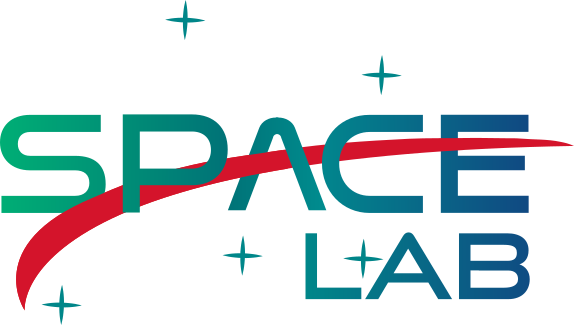
\includegraphics[width=5cm]{figures/LogotipoSpaceLab.png}
    \end{flushleft}
\end{figure}

\begin{flushleft}
\Huge{\textbf{\thetitle}}
\rule[0pt]{\textwidth}{5pt}
\end{flushleft}

\vspace{0.2cm}

\begin{flushleft}
\textit{Memory Expansion Daughterboard Documentation} \\
\textit{SpaceLab, Universidade Federal de Santa Catarina, Florianópolis - Brazil}
\end{flushleft}

\vfill
\vfill

\begin{flushright}
June 2020
\end{flushright}

\end{titlepage}

    \cleardoublepage
    %
% authorpage.tex
%
% Copyright © 2020 by Universidade Federal de Santa Catarina.
%
% Memory Expansion Daughterboard of OBDH 2.0
%
% This work is licensed under the Creative Commons Attribution-ShareAlike 4.0
% International License. To view a copy of this license,
% visit http://creativecommons.org/licenses/by-sa/4.0/.
%

%
% \brief: Author page.
%
% \author: Yan Castro de Azeredo <yan.ufsceel@gmail.com>
%
% \institution: Universidade Federal de Santa Catarina (UFSC)
%
% \version: 0.1.0
%
% \date: 09/06/20 (DD/MM/YY)
%
%  Credits to Gabriel Mariano Marcelino <gabriel.mm8@gmail.com> for the creation of this template
%
\thispagestyle{empty}

\begin{center}

\textbf{\thetitle}

\textit{June, 2020}

\vspace{1cm}

\textbf{Project Chief:}

Eduardo Augusto Bezerra

\vspace{1cm}

\textbf{Authors:}

Yan Castro de Azeredo \\
Author 2 \\
Author 3 \\

\vspace{1cm}

\textbf{Contributing Authors:}

Author 1 \\
Author 2 \\
Author 3 \\

\vspace{1cm}


\textbf{Revision Control:}

\end{center}

\begin{table}[!ht]
    \begin{center}
        \begin{tabular}{cL{5cm}L{5.5cm}C{2cm}}
            \toprule[1.5pt]
            \textbf{Version} & \textbf{Author} & \textbf{Changes}    & \textbf{Date} \\
            \midrule
            0.1     & Yan Castro de Azeredo    & Document creation   & 06/2020    \\
                    &                          &                     &            \\
                    &                          &                     &            \\
                    &                          &                     &            \\
                    &                          &                     &            \\
            \bottomrule[1.5pt]
        \end{tabular}
    \end{center}
\end{table}

\vfill

\begin{figure}[!h]
	\begin{center}
		\includegraphics[width=0.25\textwidth]{figures/by-sa.eps}
	\end{center}
\end{figure}

\textcopyright\  2020 by Universidade Federal de Santa Catarina. Memory Expansion Daughterboard of OBDH 2.0. This work is licensed under the Creative Commons Attribution-ShareAlike 4.0 International License. To view a copy of this license, visit \href{http://creativecommons.org/licenses/by-sa/4.0/}{http://creativecommons.org/licenses/by-sa/4.0/}.
    \cleardoublepage

    \listoffigures
    \addcontentsline{toc}{chapter}{List of Figures}

    \listoftables
    \addcontentsline{toc}{chapter}{Lista of Tables}

    \printnomenclature
    \addcontentsline{toc}{chapter}{Nomenclature}

    \tableofcontents
    \cleardoublepage
    
    \pagenumbering{arabic}
    \setcounter{page}{1}

    %
% introduction.tex
%
% Copyright © 2020 by Universidade Federal de Santa Catarina.
%
% Memory Expansion Daughterboard of OBDH 2.0
%
% This work is licensed under the Creative Commons Attribution-ShareAlike 4.0
% International License. To view a copy of this license,
% visit http://creativecommons.org/licenses/by-sa/4.0/.
%

%
% \brief: Introduction file.
%
% \author: Yan Castro de Azeredo <yan.ufsceel@gmail.com>
%
% \institution: Universidade Federal de Santa Catarina (UFSC)
%
% \version: 0.1.0
%
% \date: 09/06/20 (DD/MM/YY)
%
%  Credits to Gabriel Mariano Marcelino <gabriel.mm8@gmail.com> for the creation of this template
%

\chapter{Introduction} \label{ch:introduction}

The Memory Expansion Daughterboard (DB Memory in short) is a expansion module for the On-Boad-Data-Handling (OBDH 2) 
of FloripaSat-2 2U CubeSat. The main purpose of DB Memory is to give more 1gb non-volatile flash memory 
though an integrated circuit (MT25QL01GBBB) and more if added a micro sd card. 
While the module is not intended to go for flight in GOLDS-UFSC mission, 
the project had the main purpose to design the first board using the stadar SpaceLab daughter and motherboard relation 
and to serve as a prototype and testing printed circuit boards (PCB) for new comers in SpaceLab laboratory.

\begin{figure}[!ht]
    \begin{center}
        \includegraphics[width=0.75\textwidth]{figures/DifferentView_DB_Memory.png}
        \caption{3D view of the DB Memory PCB.}
        \label{fig:pcb-3d-DifferentView}
    \end{center}
\end{figure}
    %
% system_overview.tex
%
% Copyright © 2020 by Universidade Federal de Santa Catarina.
%
% Memory Expansion Daughterboard of OBDH 2.0
%
% This work is licensed under the Creative Commons Attribution-ShareAlike 4.0
% International License. To view a copy of this license,
% visit http://creativecommons.org/licenses/by-sa/4.0/.
%

%
% \brief: System overview chapter.
%
% \author: Yan Castro de Azeredo <yan.ufsceel@gmail.com>
%
% \institution: Universidade Federal de Santa Catarina (UFSC)
%
% \version: 0.1.0
%
% \date: 09/06/20 (DD/MM/YY)
%
%  Credits to Gabriel Mariano Marcelino <gabriel.mm8@gmail.com> for the creation of this template
%

\chapter{System Overview} \label{ch:system_overview}

\section{Block Diagram}

\begin{figure}[!ht]
    \begin{center}
        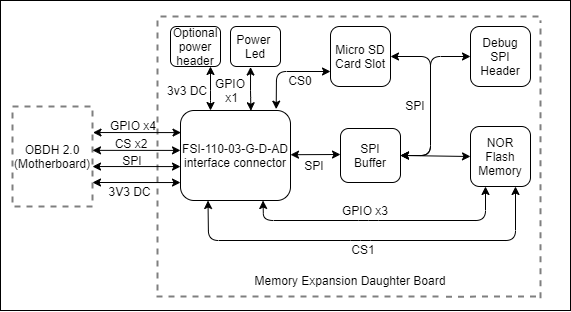
\includegraphics[width=0.75\textwidth]{figures/Architecture_Memory_Expansion_DB.png}
        \label{fig:block-diagram}
    \end{center}
\end{figure}
    %
% hardware.tex
%
% Copyright © 2020 by Universidade Federal de Santa Catarina.
%
% Memory Expansion Daughterboard of OBDH 2.0
%
% This work is licensed under the Creative Commons Attribution-ShareAlike 4.0
% International License. To view a copy of this license,
% visit http://creativecommons.org/licenses/by-sa/4.0/.
%

%
% \brief: Hardware chapter.
%
% \author: Yan Castro de Azeredo <yan.ufsceel@gmail.com>
%
% \institution: Universidade Federal de Santa Catarina (UFSC)
%
% \version: 0.1.0
%
% \date: 09/06/20 (DD/MM/YY)
%
%  Credits to Gabriel Mariano Marcelino <gabriel.mm8@gmail.com> for the creation of this template
%

\chapter{Hardware} \label{ch:hardware}

\begin{figure}[!ht]
    \begin{center}
        \includegraphics[width=0.75\textwidth]{figures/TopView_DB_Memory.png}
        \caption{Top 3D view of the DB Memory PCB.}
        \label{fig:pcb-3d-TopView}
    \end{center}
\end{figure}

\begin{figure}[!ht]
    \begin{center}
        \includegraphics[width=0.75\textwidth]{figures/BottomView_DB_Memory.png}
        \caption{Bottom 3D view of the DB Memory PCB.}
        \label{fig:pcb-3d-BottomView}
    \end{center}
\end{figure}
    %
% firmware.tex
%
% Copyright © 2020 by Universidade Federal de Santa Catarina.
%
% Memory Expansion Daughterboard of OBDH 2.0
%
% This work is licensed under the Creative Commons Attribution-ShareAlike 4.0
% International License. To view a copy of this license,
% visit http://creativecommons.org/licenses/by-sa/4.0/.
%

%
% \brief: Firmware chapter.
%
% \author: Yan Castro de Azeredo <yan.ufsceel@gmail.com>
%
% \institution: Universidade Federal de Santa Catarina (UFSC)
%
% \version: 0.1.0
%
% \date: 09/06/20 (DD/MM/YY)
%
%  Credits to Gabriel Mariano Marcelino <gabriel.mm8@gmail.com> for the creation of this template
%

\chapter{Firmware} \label{ch:firmware}
    %
% usage_instructions.tex
%
% Copyright © 2020 by Universidade Federal de Santa Catarina.
%
% Memory Expansion Daughterboard of OBDH 2.0
%
% This work is licensed under the Creative Commons Attribution-ShareAlike 4.0
% International License. To view a copy of this license,
% visit http://creativecommons.org/licenses/by-sa/4.0/.
%

%
% \brief: Usage instructions chapter.
%
% \author: Yan Castro de Azeredo <yan.ufsceel@gmail.com>
%
% \institution: Universidade Federal de Santa Catarina (UFSC)
%
% \version: 0.1.0
%
% \date: 09/06/20 (DD/MM/YY)
%
%  Credits to Gabriel Mariano Marcelino <gabriel.mm8@gmail.com> for the creation of this template
%

\chapter{Usage Instructions} \label{ch:usage_instructions}
    %
% references.tex
%
% Copyright © 2020 by Universidade Federal de Santa Catarina.
%
% Memory Expansion Daughterboard of OBDH 2.0
%
% This work is licensed under the Creative Commons Attribution-ShareAlike 4.0
% International License. To view a copy of this license,
% visit http://creativecommons.org/licenses/by-sa/4.0/.
%

%
% \brief: References chapter.
%
% \author: Yan Castro de Azeredo <yan.ufsceel@gmail.com>
%
% \institution: Universidade Federal de Santa Catarina (UFSC)
%
% \version: 0.1.0
%
% \date: 09/06/20 (DD/MM/YY)
%
%  Credits to Gabriel Mariano Marcelino <gabriel.mm8@gmail.com> for the creation of this template
%

%\bibliography{references/*.bib}

\addcontentsline{toc}{chapter}{References}

\end{document}